% Formatting draft for JIRS; NOT SUBMITTED. Author fields intentionally blank.
% The official sn-jnl.cls is unchanged. No custom fonts. One manuscript TeX.
\documentclass[pdflatex,sn-mathphys-num]{sn-jnl}
\usepackage{graphicx,amsmath,amssymb,booktabs,array,textcomp}
\hypersetup{colorlinks=true,linkcolor=black,citecolor=black,urlcolor=blue,pdfauthor={}}
\setlength{\emergencystretch}{3em}
\newlength{\JournalTableWidth}
\providecommand{\tightlist}{\setlength{\itemsep}{0pt}\setlength{\parskip}{0pt}}
\providecommand{\passthrough}[1]{#1}
\providecommand{\pandocbounded}[1]{#1}
\raggedbottom
\begin{document}
\title{Category Priors and Geometric Feedback for Budget-Constrained Active Observation of Facilities}
% Author name, affiliation, email and ORCID: deliberately not supplied.
% \author*[1]{\fnm{} \sur{}}\email{}
% \affil*[1]{\orgdiv{},\orgname{},\orgaddress{\city{},\country{}}}
\abstract{Industrial robots need current environmental representations after equipment rearrangement, but spatial coverage alone does not ensure adequate surface reconstruction. This study investigates category information for selecting observation directions before geometry resolves a facility configuration. A processor-based implementation connects category-conditioned beliefs, diagnostic lookahead, execution checks, and measured feedback. Public templates predict opportunities; only acquired depth contributes to reconstruction. In a confirmation using two previously seen layouts and two configurations each, category information improves the mean product of coverage and surface F1 score by 6.1638\%, with two wins, two ties, and identical mean coverage. A frozen-policy validation in two additional background layouts yields one win and three ties, improving the mean joint score by 2.9818\% across four paired conditions. An incorrect-prior comparison supports a 2.6241\% improvement from the complete correction policy. A fixed 128-trial extension yields 96 qualified completions and 32 low-budget planning failures. At the intermediate budget, category gains are 6.2505\% on original layouts and 4.2289\% on same-family variants; at the larger budget, the original-layout difference reverses to \ensuremath{-}0.6995\%. Forty reconstruction checkpoints connect these outcomes to measured surface recovery. A separate 36-run multi-facility study gives identical actions and quality for shared versus fixed category priors in all nine version-specific pairs. The evidence supports conditional benefits from early category cues, without establishing additional sharing or localization-accuracy gains.}
\keywords{active observation, facility documentation, category priors, geometric feedback, budget-constrained reconstruction}
\maketitle
\noindent\textbf{Categories:} (2), (5), (8).\quad\textit{Formatting draft; not submitted.}

\hypertarget{introduction}{%
\section{Introduction}\label{introduction}}

Industrial embodied systems depend on current environmental representations \cite{ref9}. Equipment rearrangement, workstation changes, and material relocation can invalidate a previously useful map. A robot may then need to reacquire the accessible layout and document nearby equipment. We consider a static environment during each acquisition task; changes occur between tasks, and dynamic obstacle avoidance is outside the scope.

Active mapping selects motion to improve an environmental model \cite{ref10}. For facility documentation, two objectives interact: observing the surrounding space and obtaining sufficient views of equipment surfaces. A robot can traverse a corridor and observe most of its accessible area while missing a recessed face or a structure on the far side of a cabinet. Additional travel through already visible open space may contribute little to that missing geometry. Under a finite action budget, the observation side and the timing of a turn can therefore matter as much as the distance traveled.

Categories may provide useful information before geometric disambiguation. If a recognized category is associated with an opening or service-side configuration, it can favor an observation route while the initial depth measurements remain ambiguous. This advantage is not automatic. An active geometric planner can also purchase a diagnostic view, revisit a location, and redirect its route. An incorrect category cue can waste the remaining budget unless contrary measurements change the belief and action. A meaningful semantic comparison must therefore retain active geometric planning in the control.

We ask whether a category cue can reduce the cost of selecting a useful observation direction under common navigation, reconstruction, and planning resources. This study makes three contributions:

\begin{enumerate}
\def\labelenumi{\arabic{enumi}.}
\tightlist
\item
  A category-conditioned observation method connects configuration priors, diagnostic lookahead, return constraints, and measured reconstruction in a planning--execution loop. A matched geometric control retains the same diagnosis, revisiting, and reconstruction capabilities, isolating the additional category information.
\item
  A two-configuration decision analysis relates category confidence, diagnostic cost, and directional utility. Recorded decisions and same-state posterior interventions explain how category cues select an early direction and how measured geometry corrects misleading priors.
\item
  Paired trajectories, actual TSDF meshes, fixed reconstruction checkpoints, and budget/geometry variations connect decision changes to measured surface recovery and identify the conditions under which category benefits persist or disappear.
\end{enumerate}

The contribution is a task-specific observation method and its mechanism evidence. Bayesian updating and semantic inspection provide established foundations. A separate multi-facility implementation examines the limits of sharing class-model evidence.

\hypertarget{related-work}{%
\section{Related Work}\label{related-work}}

Active Neural SLAM provides an early learned hierarchical exploration architecture \cite{ref1}; this project retains the general decision/execution separation while replacing the mechanism and task. TARE coordinates local and global exploration through representations at different resolutions \cite{ref5}. The active-SLAM survey by Placed et al.~connects motion selection, map quality, and estimation \cite{ref10}. Here, exact poses and a common safe graph isolate observation allocation rather than localization accuracy.

Next-best-view methods select observations to improve reconstruction. GenNBV learns a policy using geometric, semantic, and action representations in a five-dimensional viewpoint space \cite{ref6}. Our implementation instead uses a finite public configuration family and discrete ground motion. Both internal policies can seek informative geometry. Their reconstruction backend uses Open3D \cite{ref4} and volumetric range integration \cite{ref11}, with measured depth as the sole source of surfaces. This separates using a prior to decide where to look from using it to complete an unobserved surface.

Semantic inspection already connects target meaning with observation requirements. SWAP combines exploration, semantic completion, and surface inspection \cite{ref2}, while semantics-aware predictive inspection planning uses repeated structures in semantic scene graphs to anticipate unseen inspection targets \cite{ref7}. VISTA combines task relevance and directional coverage in online semantic Gaussian mapping \cite{ref3}, and ActiveSGM couples semantic and geometric uncertainty when predicting observation informativeness \cite{ref8}. These works motivate information-aware allocation; semantic revisiting and structural prediction are not claimed as new concepts here.

These methods connect semantics to target requirements, repeated structures, query relevance, or uncertainty. Here, the category variable conditions an explicit hypothesis about a facility's hidden configuration. We examine when this prior changes the choice between return-feasible observation routes and how acquired geometry revises that choice. Belief-based decisions and informative path planning supply established foundations \cite{ref12,ref13}. SWAP-I/VISTA-I comparisons adapt selected mechanisms to common candidates and fusion; native TARE integration provides engineering evidence. The primary category contrast uses matched internal planners, while the adapted comparisons do not represent complete-system state-of-the-art rankings.

\hypertarget{task-information-and-quality}{%
\section{Task, Information, and Quality}\label{task-information-and-quality}}

The local task contains one facility with an unknown configuration \(h\in\{0,1\}\). Both policies receive two public templates, a facility coordinate frame, an initial pose \(s_0\), and a safe pose graph. They receive RGB-D, planar scan, and pose observations only when those observations are acquired. The category--configuration association is manually specified public knowledge. Evaluation references, true configuration identifiers, and actual measurements from unexecuted actions are unavailable to the planner.

A forward motion of 1 m or a 90\ensuremath{^{\circ}} turn consumes one action and acquires a sensor frame. An identical 18-action observation prefix precedes autonomous selection within total budget \(B\). The original confirmation uses \(B=42\); the extension also evaluates 30 and 54. A qualified task must remain collision-free, finish within budget, attain at least 80\% planar coverage, and return to the initial position and orientation. The experiment consequently tests allocation after common observation, rather than unknown-environment exploration from the first action.

The principal measured score combines planar coverage and surface quality:

\[
C_{\rm map}=\frac{|\{c\in\mathcal R:m_T(c)\ne-1\}|}{|\mathcal R|},
\qquad F_{1,\tau}=\frac{2P_\tau R_\tau}{P_\tau+R_\tau},
\qquad J_5=C_{\rm map}F_{1,0.05}.
\]

The evaluator derives the start-reachable safe-cell set \(\mathcal R\) using a 0.2 m grid and 0.2 m robot radius. It contains 588 cells in P00 and 668 in P01. A nonunknown cell counts as observed, including one marked occupied, so coverage is not occupancy-classification accuracy. Ground truth is used after prediction sealing, not to supply runtime measurements.

Surface precision and recall follow distance-threshold comparison \cite{ref14}. Precision queries the reference from sampled predicted surfaces; recall queries the prediction from fixed exterior vertical reference surfaces. The prediction is cropped to the common bounding box of both templates with a 0.20 m margin, and the known ground is removed. Thus, errors outside this region do not enter precision. No registration or hole filling is applied. Thresholds are fixed at 2, 5, and 10 cm, with 5 cm primary; empty predictions receive zero quality. Coverage, precision, recall, and task qualification accompany the product to avoid hiding its components.

The desired policy maximizes expected measured \(J_5\) using acquired information while respecting budget and return constraints. Online template exposure is only its planning surrogate. A larger predicted opportunity need not produce a more accurate fused mesh, and additional observations do not guarantee improvement at every surface threshold.

\hypertarget{observation-planning-with-correctable-category-priors}{%
\section{Observation Planning with Correctable Category Priors}\label{observation-planning-with-correctable-category-priors}}

\hypertarget{executable-module-interfaces}{%
\subsection{Executable module interfaces}\label{executable-module-interfaces}}

The decision layer selects an observation subgoal, and the execution layer checks its legality and return cost. In the local implementation, that subgoal is the next atomic action. Four interfaces connect the acquired evidence to this decision (Table 1 and Figure 1). Their names describe responsibilities in the CPU prototype, not four independently validated learned networks. The geometric control G and category-conditioned S use the same planner, public predictions, safe graph, and reconstruction backend; G can actively diagnose configurations and revisit locations.

\begin{table}[!htbp]
\caption{Four CPU interfaces and their executed roles}\label{tab:1}
\small\setlength{\tabcolsep}{3pt}
\setlength{\JournalTableWidth}{\dimexpr\linewidth-4\tabcolsep\relax}
\begin{tabular}{@{}>{\raggedright\arraybackslash}p{0.16\JournalTableWidth} >{\raggedright\arraybackslash}p{0.32\JournalTableWidth} >{\raggedright\arraybackslash}p{0.52\JournalTableWidth}@{}}
\toprule
Interface & Input & Output and role \\
\midrule
OV-SDF & Acquired RGB, pose, measured-map summary & Register category support and configuration prior \\
STGHP & Graph, exposure sets, beliefs, remaining budget & Compare feasible continuations and select a subgoal \\
RPN-UQ & Proposed edge, budget, return distance & Permit or reject the executable action \\
IGCR & Acquired depth/scan and public predictions & Bound geometric evidence and revise belief \\
\bottomrule
\end{tabular}
\end{table}

\begin{figure}[!htbp]
\centering
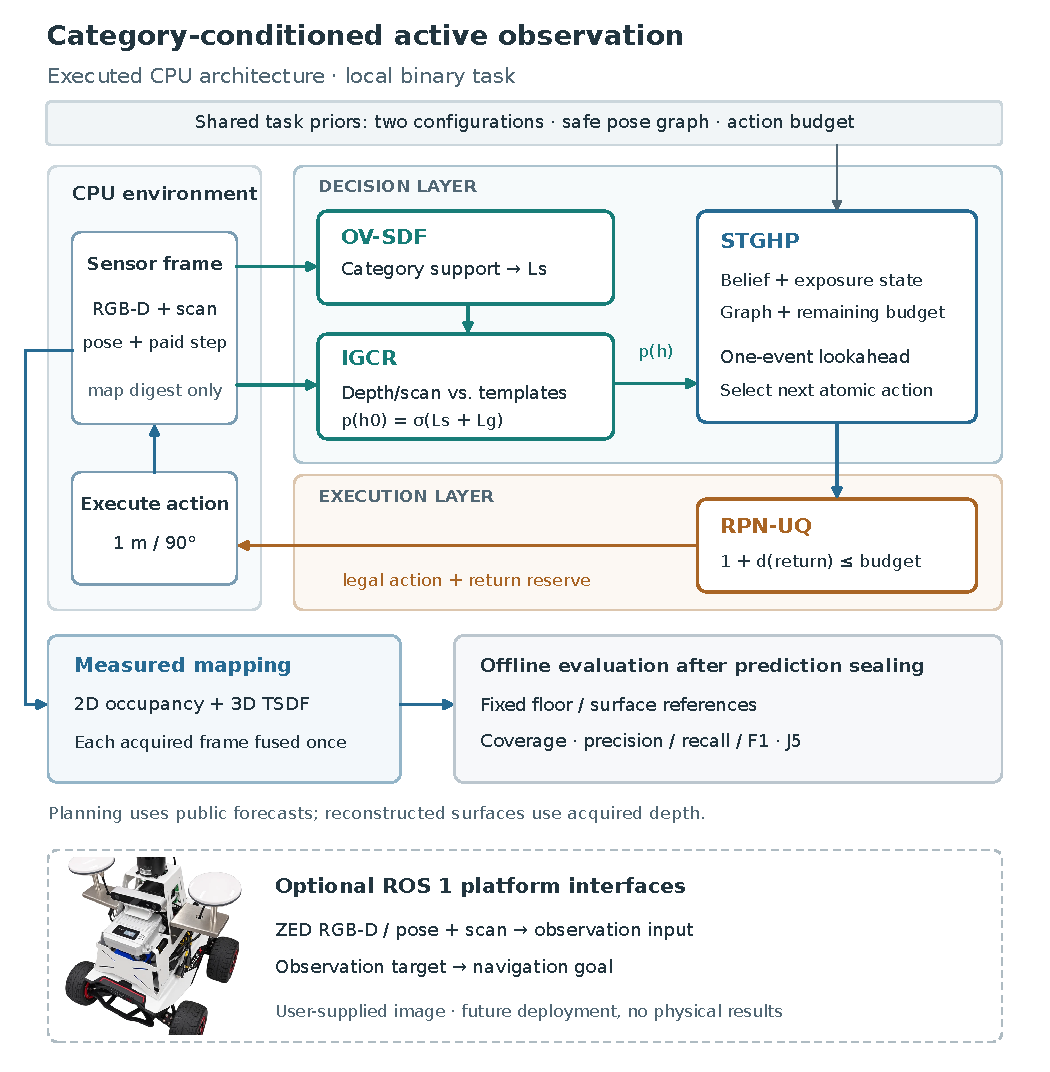
\includegraphics[width=\linewidth,height=.67\textheight,keepaspectratio]{Fig1.pdf}
\caption{CPU observation and execution architecture. Category and geometric evidence update the belief used for planning; acquired depth separately enters TSDF fusion. The unchanged user-supplied robot image illustrates prospective ROS 1 interfaces. All reported performance is simulated; the diagram uses programmatically drawn vector elements}\label{fig:1}
\end{figure}

\hypertarget{measured-evidence-and-correction}{%
\subsection{Measured evidence and correction}\label{measured-evidence-and-correction}}

Let \(L_t^g\) be cumulative geometric support and \(L_t^s\) category support for configuration 0. Its planning weight is

\[
L_t^g=\operatorname{clip}_{[-24,24]}(L_{t-1}^g+\delta_t),
\qquad p_t=\sigma(L_t^g+L_t^s).
\]

Category registration requires at least 16 exact-color pixels at each of two distinct XY positions, with no competing marker color in those frames. It assigns \(L_t^s=\pm\log9\); repeated observations do not multiply the prior, and conflicting registrations clear it. G sets \(L_t^s=0\). These synthetic markers isolate category availability without claiming natural recognition accuracy.

At a newly visited pose, geometric evidence is the mean loss difference \(e_1-e_0\), clipped to \([-6,6]\), over eligible depth and scan modalities. Residuals are computed where the public predictions differ. Depth requires eight valid pixels and uses normalized disparity residual \((57.6/z-57.6/\widehat z_h)/0.25\); scan requires three valid beams and uses \((r-\widehat r_h)/0.02\). Each loss is half the squared residual, capped at 12.5. Missing measured returns do not provide evidence. Repeated poses add no further belief increment, although newly acquired depth still enters fusion. The support weights are uncalibrated pseudo-likelihoods; rejecting exact repeats does not establish independence of nearby views.

An incorrect finite prior can be overturned. If \(L^s>0\) favors configuration 0, obtaining support at least \(\eta>1/2\) for configuration 1 requires

\[
L_t^g\le-L^s-\operatorname{logit}(\eta).
\]

This threshold describes the implemented weights, subject to the cumulative cap and availability of informative measurements. It is not a guarantee of calibrated confidence or improved reconstruction.

\hypertarget{diagnostic-lookahead-costs-and-measured-fusion}{%
\subsection{Diagnostic lookahead, costs, and measured fusion}\label{diagnostic-lookahead-costs-and-measured-fusion}}

The planning state contains pose, remaining budget, belief, visited poses, and separate template exposure sets \(M_0,M_1\). A stopping state must be at the initial pose and have predicted coverage at least 0.8 under both templates. Its value is \(p\widetilde J_0(M_0)+(1-p)\widetilde J_1(M_1)\), where \(\widetilde J_h\) multiplies predicted ground exposure and exposed exterior surface fraction. Template geometry is never inserted into the measured mesh.

Dynamic programming compares executable continuations with at most one future diagnostic event per planning call. At an unobserved diagnostic node, the forecast branches under assumed diagnostic accuracy \(r=0.99\):

\[
\lambda_0=pr+(1-p)(1-r),\qquad
p^{(0)}=\frac{pr}{\lambda_0},\qquad
p^{(1)}=\frac{p(1-r)}{1-\lambda_0}.
\]

The expected continuation combines the two branch values; no further diagnostic event is expanded within that call. Diagnostic nodes are identified from differences between the public templates, and both branches must remain feasible. Only the first action is executed before replanning from acquired evidence. Forecast weights never replace the measured belief. The category strength 0.9 and forecast setting 0.99 are fixed design choices shared across comparisons, not measured recognition or sensor reliability.

For action cost one, RPN-UQ requires \(1+d_{\rm return}(s')\le b_t\), where return includes starting orientation. On the fixed legal graph, this preserves an affordable return path by induction. It does not guarantee recovery from collision or computation failure. Planning is limited to 1.5 million cached states and approximately 20 s per call; the exposure-state dependence remains exponential. Thus, the implementation makes no claim of scalable optimal planning for measured reconstruction quality.

Each execution produces a frame that is fused exactly once using the shared CPU TSDF backend, with 4 cm voxels and 12 cm truncation. The controller then updates category support, geometric evidence, exposure sets, and remaining budget. Stopping, infeasibility, and forced termination are distinguished. Reconstruction and action records are sealed before endpoint evaluation.

\hypertarget{why-a-cue-can-save-observation-budget}{%
\subsection{Why a cue can save observation budget}\label{why-a-cue-can-save-observation-budget}}

A simple decision model identifies the mechanism. Assume two initially indistinguishable, equally likely configurations and two return-feasible routes. A correctly matched route yields utility \(U_+\), an unmatched route \(U_-\), and \(\Delta=U_+-U_->0\). A category cue has symmetric reliability \(r_c\ge1/2\); an optional geometric diagnosis has symmetric reliability \(r_d\ge1/2\), conditional independence given configuration, and utility cost \(\kappa\ge0\). Both routes remain feasible afterward. For current probability \(p\), diagnosis improves route-selection accuracy from \(m=\max(p,1-p)\) to \(\max(m,r_d)\). Its net value is therefore

\[
\Delta\max(0,r_d-m)-\kappa.
\]

G purchases diagnosis when \(\kappa<(r_d-1/2)\Delta\), while a policy following the cue needs \(\kappa<(r_d-r_c)_+\Delta\). Category information can save a diagnostic detour when it already supplies enough directional confidence. The advantage vanishes if geometry resolves the configuration, route values coincide, or diagnosis is sufficiently cheap. These established decision principles \cite{ref12,ref13} explain a possible mechanism; they neither establish a new Bayesian algorithm nor predict every TSDF outcome.

\hypertarget{experiments-and-results}{%
\section{Experiments and Results}\label{experiments-and-results}}

\hypertarget{protocol-and-comparisons}{%
\subsection{Protocol and comparisons}\label{protocol-and-comparisons}}

The simulator supplies 96\ensuremath{\times}72 depth images over a 4 m range and a 360\ensuremath{^{\circ}} planar scan with 180 beams over 8 m. Poses are exact. Depth noise has a standard deviation of 0.25 pixels in reference disparity; no additional random scan noise is applied. The experiments isolate planning under controlled observations rather than reproduce physical sensor errors.

Confirmation freezes the controller and uses a held-out noise seed on two previously seen parent layouts, each with two configurations: eight runs and four G/S pairs. Separate development comparisons use incorrect category interpretation X and Xnf, which also disables measured correction and future diagnostic anticipation. Their contrast evaluates the whole correction policy. Replays and alternative thresholds reuse these trajectories; they do not increase the number of independent layouts or trials. All controls retain active geometric reasoning.

The recorded software is Python 3.12.3, NumPy 1.26.4, SciPy 1.11.4, and Open3D 0.19.0, with one OpenMP, OpenBLAS, and MKL thread. No GPU is required. Figures use actual recorded actions and measured meshes except the explicitly schematic architecture diagram.

\begin{figure}[!htbp]
\centering
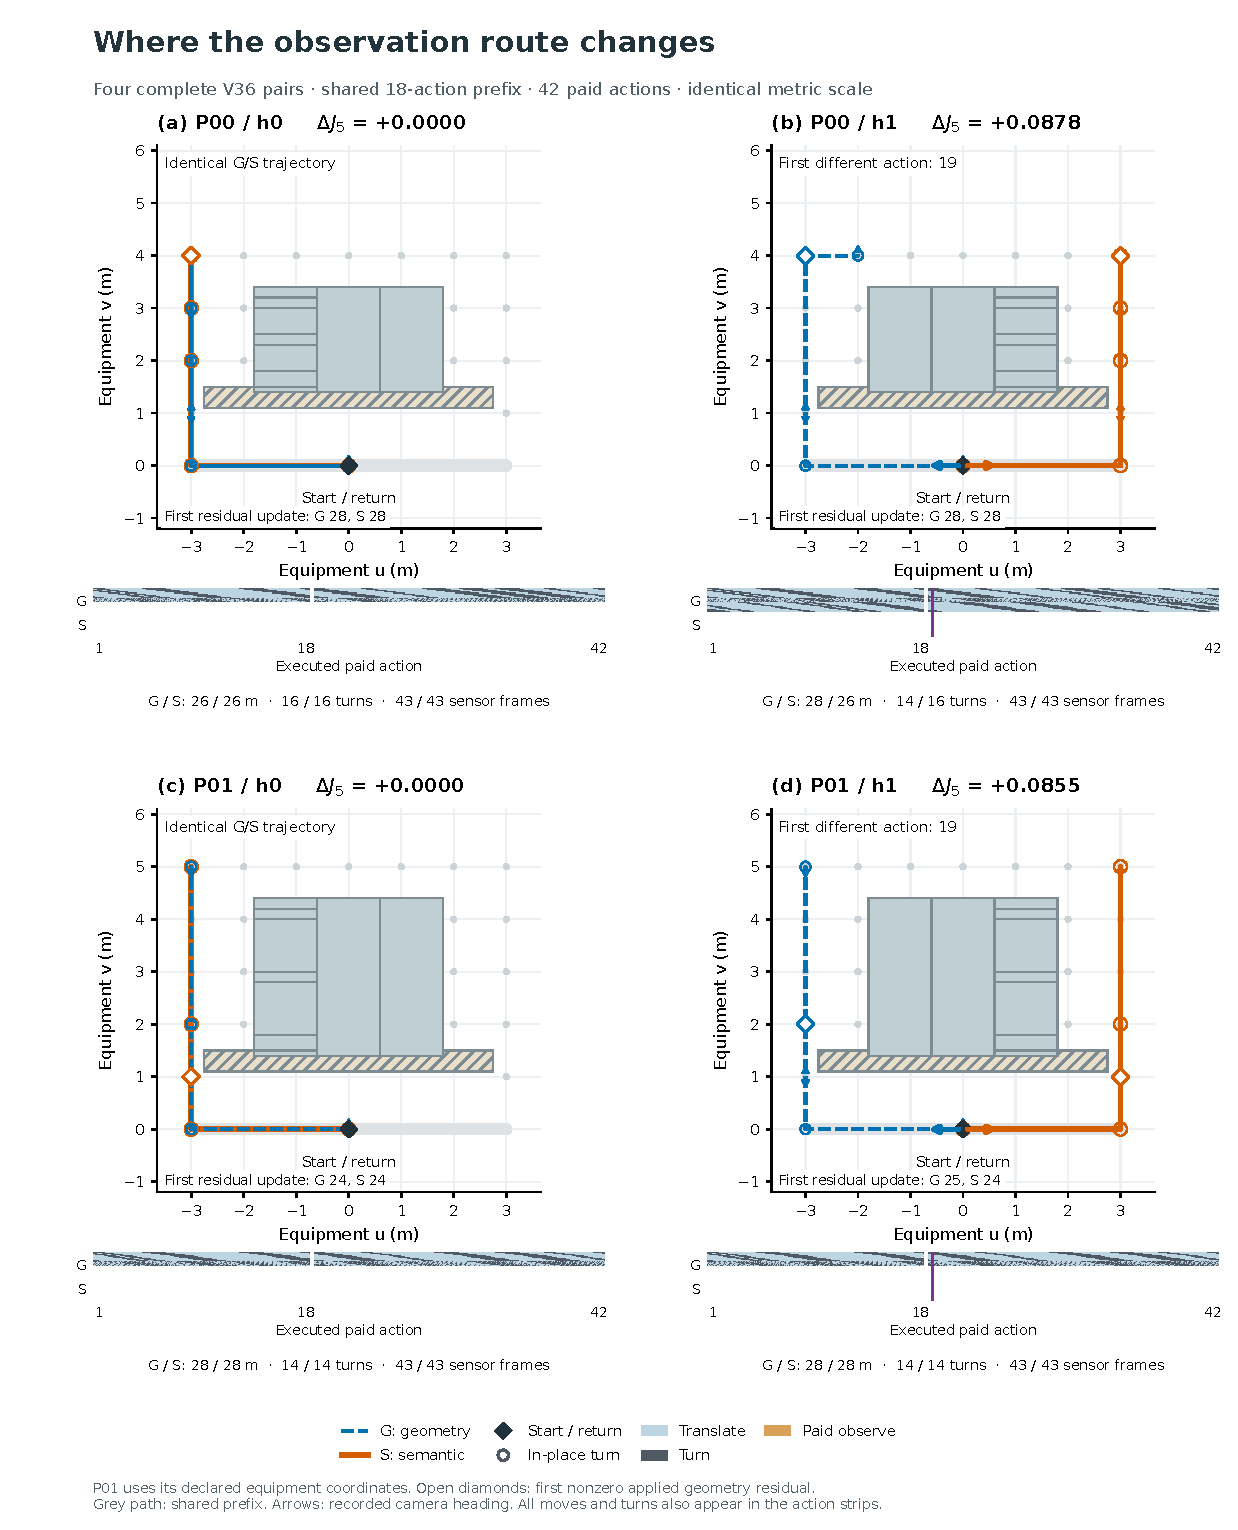
\includegraphics[width=\linewidth,height=.67\textheight,keepaspectratio]{Fig2.pdf}
\caption{Both configurations of P00 and P01, with common 18-action prefixes, saved paths, and complete action strips. Panels share metric scale. Circles denote turns, arrows recorded headings, and open diamonds first applied geometric feedback. The two h0 routes coincide; both h1 pairs diverge at action 19}\label{fig:2}
\end{figure}

\hypertarget{category-information-changes-observed-surfaces}{%
\subsection{Category information changes observed surfaces}\label{category-information-changes-observed-surfaces}}

Table 2 retains all four confirmation pairs. Mean \(J_5\) increases from 0.702576 to 0.745881, a relative improvement of \textbf{6.1638\%}, with two wins and two ties. Every run uses 42 actions, avoids collision, and returns exactly. Mean coverage is identical at 0.952544; mean surface F1 increases from 0.737490 to 0.782951. The gain is therefore a surface-quality improvement at matched coverage, not a localization improvement.

\begin{table}[!htbp]
\caption{Complete confirmation pairs; relative change compares policy means}\label{tab:2}
\small\setlength{\tabcolsep}{3pt}
\setlength{\JournalTableWidth}{\dimexpr\linewidth-6\tabcolsep\relax}
\begin{tabular}{@{}>{\raggedright\arraybackslash}p{0.32\JournalTableWidth} >{\raggedright\arraybackslash}p{0.22\JournalTableWidth} >{\raggedright\arraybackslash}p{0.22\JournalTableWidth} >{\raggedright\arraybackslash}p{0.24\JournalTableWidth}@{}}
\toprule
Layout/configuration & G: \(J_5\) & S: \(J_5\) & S\ensuremath{-}G \\
\midrule
P00/h0 & 0.772200 & 0.772200 & 0 \\
P00/h1 & 0.672703 & 0.760456 & +0.087753 \\
P01/h0 & 0.727281 & 0.727281 & 0 \\
P01/h1 & 0.638118 & 0.723586 & +0.085468 \\
Mean & 0.702576 & 0.745881 & +0.043305 \\
\bottomrule
\end{tabular}
\end{table}

In both h1 cases, category conditioning changes the first autonomous turn. The resulting surface recall rises from 0.5958 to 0.7249 in P00 and from 0.5555 to 0.6845 in P01. Both h0 pairs follow identical trajectories. The relative mean gains at 2 and 10 cm are 5.5040\% and 6.2110\%, respectively. These descriptive sensitivities do not establish statistical significance across unseen layouts.

\begin{figure}[!htbp]
\centering
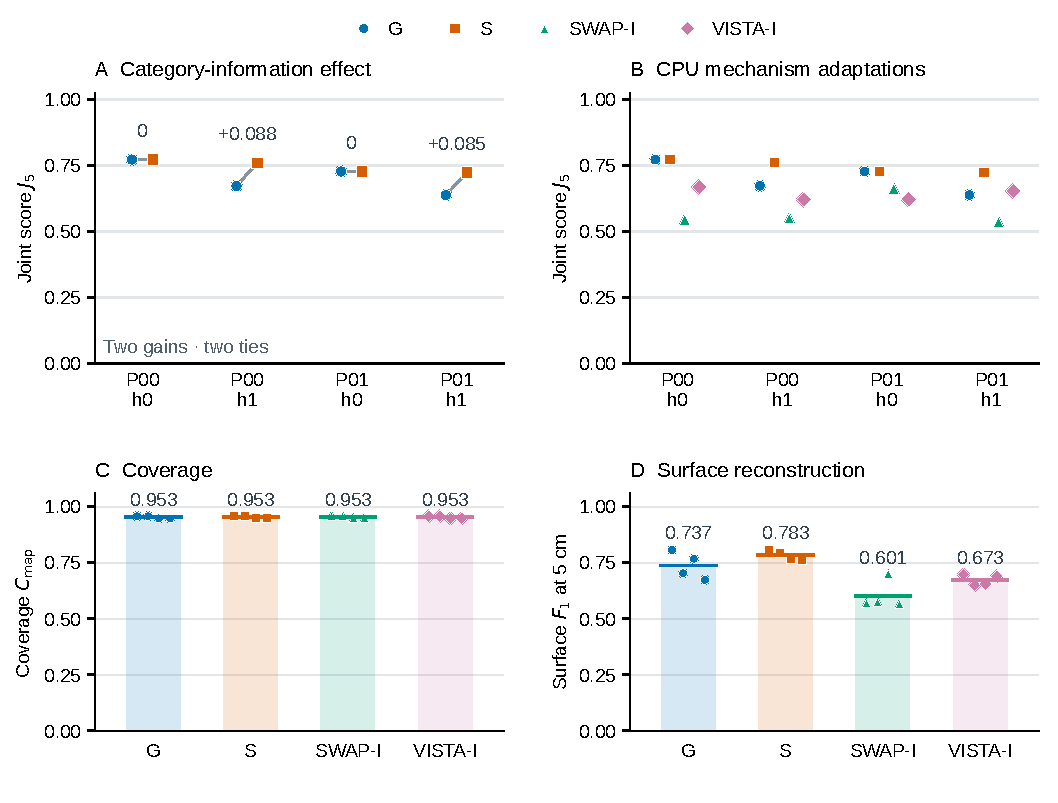
\includegraphics[width=\linewidth,height=.67\textheight,keepaspectratio]{Fig3.pdf}
\caption{Complete paired outcomes, including both ties, and the coverage/F1 decomposition. Points represent conditions; horizontal caps indicate means rather than confidence intervals. G/S trajectories reused in the external-mechanism panel are not additional evidence}\label{fig:3}
\end{figure}

Actual endpoint meshes in Figure 4 show the recovered side structures using matched cameras and scales. P00/h1 needs 28 m and 14 turns for G versus 26 m and 16 turns for S; P01/h1 uses 28 m and 14 turns for both. Every run acquires the same number of frames. The effect therefore depends on allocating observations differently, rather than increasing sensing or travel.

\begin{figure}[!htbp]
\centering
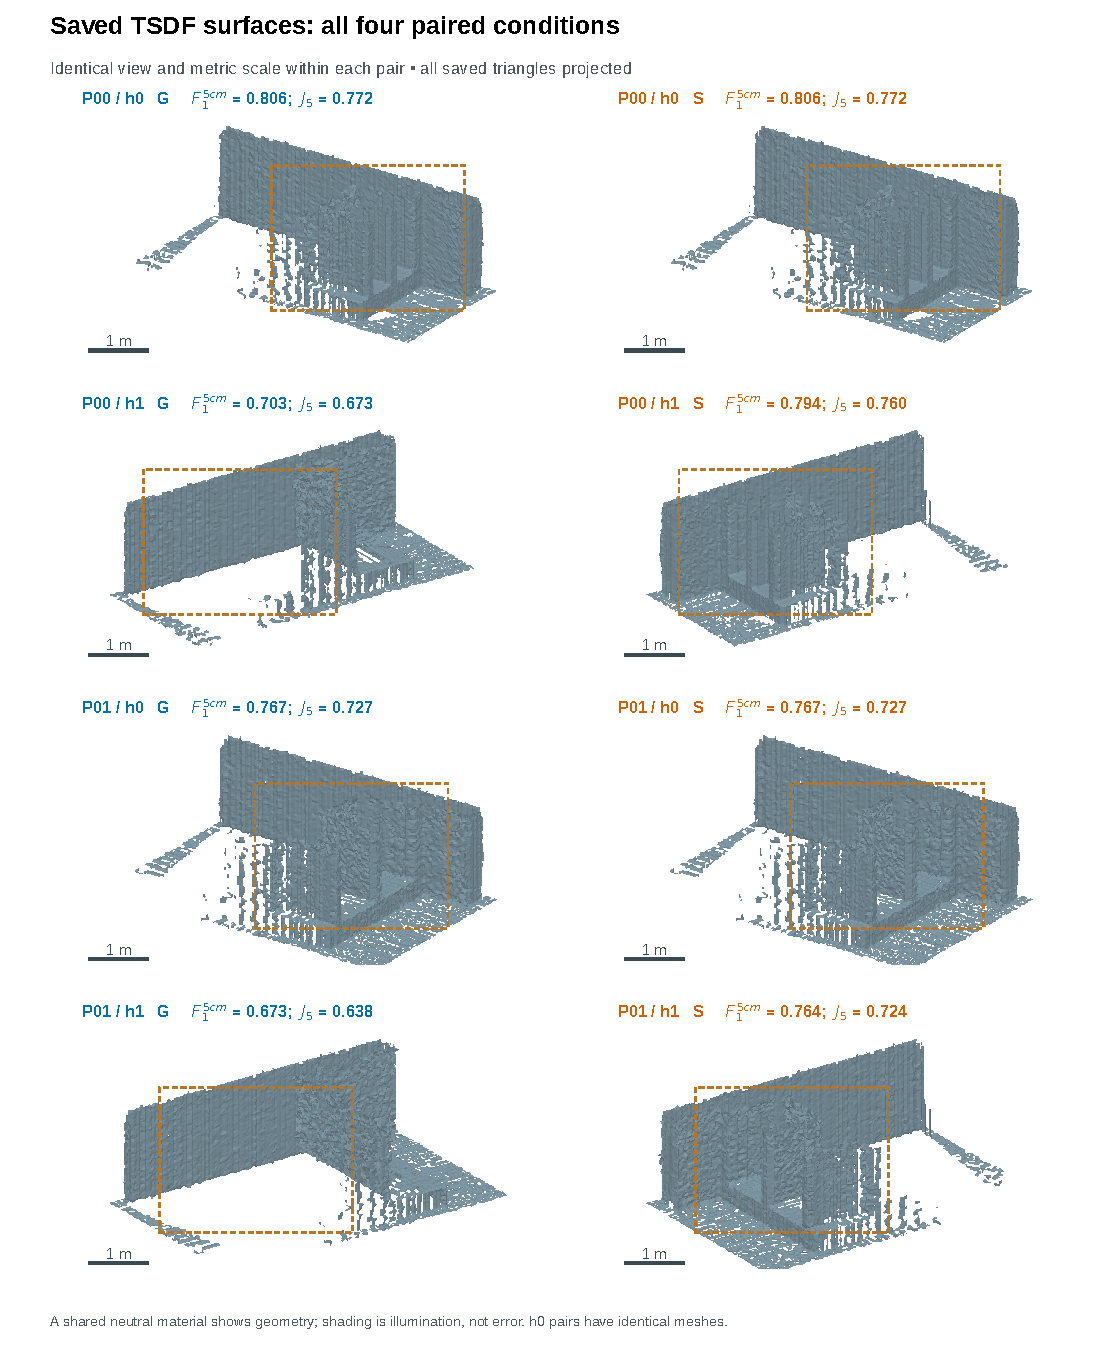
\includegraphics[width=\linewidth,height=.67\textheight,keepaspectratio]{Fig4.pdf}
\caption{Saved TSDF meshes in the common evaluation region. Each pair shares camera, scale, material, and lighting; all stored triangles are rendered. Both h0 pairs remain identical. Shading represents illumination, not error. Dashed windows correspond to matched detail views (Online Resource 1); no smoothing, template completion, or local quality score is introduced}\label{fig:4}
\end{figure}

\hypertarget{measured-correction-and-reconstruction-progress}{%
\subsection{Measured correction and reconstruction progress}\label{measured-correction-and-reconstruction-progress}}

The saved P00 development decisions explain the mechanism. After the common prefix, G assigns configuration-1 weight 0.5, and equal continuation values of 0.650944 resolve to the fixed left-turn tie rule. For h1, S assigns weight 0.9; left/right values become 0.668008/0.711865, selecting right at action 19. These are predicted continuation values, not measured F1.

With the incorrect cue, X starts from weight 0.1. At step 28, 1092 informative depth pixels produce a clipped geometric increment of \ensuremath{-}6, yielding configuration-1 support \(1-\sigma(-6+\log9)=0.978178\). Action 29 becomes forward, while Xnf turns right. Across the two development configurations, X improves mean \(J_5\) over Xnf from 0.655065 to 0.672254, or 2.6241\%. Because Xnf also removes anticipated diagnosis, this is not an isolated posterior-update ablation. At 2 cm, the h1 difference is \ensuremath{-}0.0021593573, retaining a correction boundary.

\begin{figure}[!htbp]
\centering
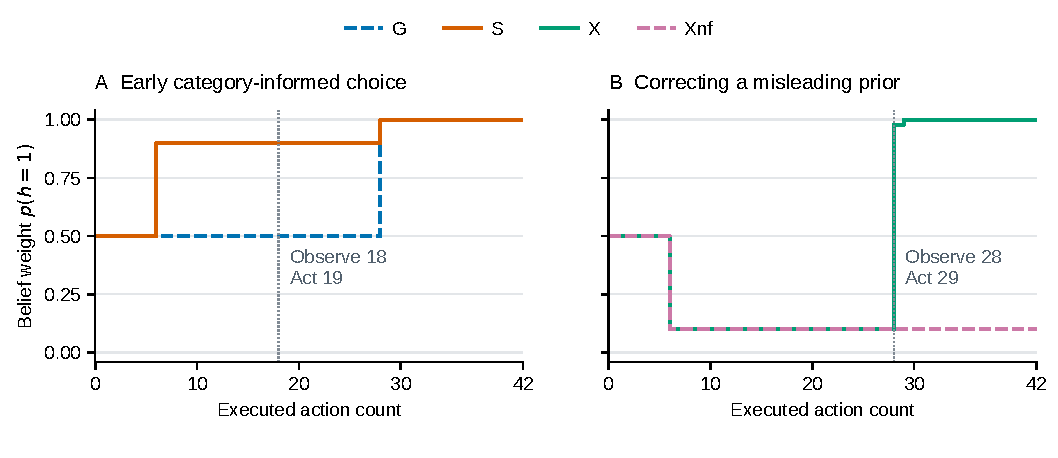
\includegraphics[width=\linewidth,height=.67\textheight,keepaspectratio]{Fig5.pdf}
\caption{Acquired category support changes action 19; contrary measured geometry at step 28 changes action 29. Curves are uncalibrated configuration weights from P00/h1 development logs. The timeline explains the decisions without adding counterfactual endpoint trials}\label{fig:5}
\end{figure}

We further reintegrate the eight saved confirmation trajectories at 18, 24, 30, 36, and 42 paid actions: \textbf{40 measured checkpoints}, with unchanged observations, poses, fusion settings, and evaluator. All 16 previously available prefix/endpoint checkpoints reproduce their original metrics exactly. Coverage matches within every pair at every checkpoint and reaches its endpoint value by action 30. Later differences mainly accompany increased surface recall and F1. P00/h1 is still slightly worse for S at action 24 (\ensuremath{-}0.000819), then positive at 30, 36, and 42; P01/h1 is already positive at 24. Both h0 pairs remain tied. Intermediate states may not satisfy return or coverage requirements and are not successful terminal trials.

\begin{figure}[!htbp]
\centering
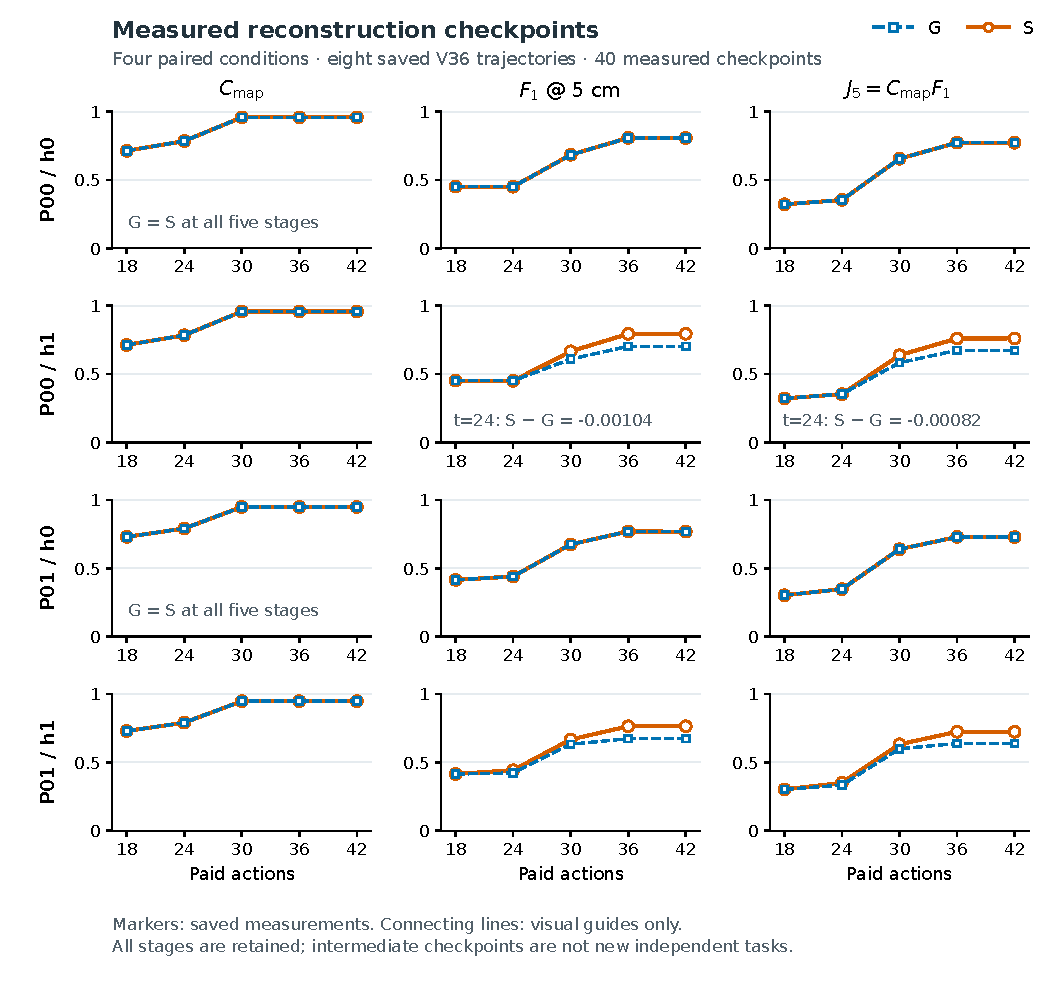
\includegraphics[width=\linewidth,height=.67\textheight,keepaspectratio]{Fig6.pdf}
\caption{Coverage, 5 cm surface F1, and joint quality for all four paired conditions at all five measured checkpoints. Markers are actual measurements; connecting lines are visual guides. Both h0 ties and the early P00/h1 negative difference remain visible, with common 0--1 axes. Forty checkpoints reuse eight trajectories and add no independent runs. Complete precision/recall figure (Online Resource 2) and actual stage meshes (Online Resource 3) accompany the data}\label{fig:6}
\end{figure}

\hypertarget{cpu-mechanism-comparisons}{%
\subsection{CPU mechanism comparisons}\label{cpu-mechanism-comparisons}}

SWAP-I and VISTA-I each complete four qualified tasks using common sensing and fusion. Table 3 summarizes their measured endpoints. Their lower scores indicate different observation allocation in this task, while changed objectives and planner details prevent attributing the full differences to category information. A native TARE node additionally completes four migration tasks, but narrow-field-of-view conversion, waypoint projection, waiting, and return depend on its adapter. Those runs establish integration feasibility rather than matched performance superiority.

\begin{table}[!htbp]
\caption{Four-condition CPU means; coverage is 0.952544 for every method}\label{tab:3}
\small\setlength{\tabcolsep}{3pt}
\setlength{\JournalTableWidth}{\dimexpr\linewidth-6\tabcolsep\relax}
\begin{tabular}{@{}>{\raggedright\arraybackslash}p{0.32\JournalTableWidth} >{\raggedright\arraybackslash}p{0.22\JournalTableWidth} >{\raggedright\arraybackslash}p{0.22\JournalTableWidth} >{\raggedright\arraybackslash}p{0.24\JournalTableWidth}@{}}
\toprule
Method & Surface F1 at 5 cm & \(J_5\) & Planner/record time (s) \\
\midrule
G & 0.737490 & 0.702576 & 0.067853 \\
S & 0.782951 & 0.745881 & 0.123555 \\
SWAP-I & 0.600887 & 0.572223 & 1.256934 \\
VISTA-I & 0.672911 & 0.640977 & 1.388679 \\
\bottomrule
\end{tabular}
\end{table}

Timing excludes sensing, fusion, and evaluation. Historical manifests do not preserve CPU model or core count, so these values are not hardware-normalized throughput claims.

\hypertarget{fixed-budget-noise-and-geometry-extension}{%
\subsection{Fixed budget, noise, and geometry extension}\label{fixed-budget-noise-and-geometry-extension}}

The fixed extension declares 128 trials. Original P00/P01, two configurations, budgets 30/42/54, two noise seeds, and four policies define 96 trials. Two same-family variants at budget 42 add 32: one P00 rib shifts 0.25 m, while three P01 ribs lower their upper boundary from 1.80 to 1.35 m. Transformations apply consistently to both public hypotheses, sensed geometry, and reference surfaces. The safe graph, prefix, controller, and prior settings remain unchanged. These variants test nearby geometry, not unseen natural equipment categories.

All 128 tasks are attempted once: 96 qualify and 32 fail at budget 30 after the common prefix. The controller cannot find a return plan meeting its predicted 80\% coverage gate under both templates. This is a planning-constraint boundary, not universal physical impossibility. Failure maps remain separate from successful endpoint means.

\begin{table}[!htbp]
\caption{Complete extension groups. Each row declares 32 trials; qualified rows contain eight per policy}\label{tab:4}
\small\setlength{\tabcolsep}{3pt}
\setlength{\JournalTableWidth}{\dimexpr\linewidth-10\tabcolsep\relax}
\begin{tabular}{@{}>{\raggedright\arraybackslash}p{0.26\JournalTableWidth} >{\raggedright\arraybackslash}p{0.148\JournalTableWidth} >{\raggedright\arraybackslash}p{0.148\JournalTableWidth} >{\raggedright\arraybackslash}p{0.148\JournalTableWidth} >{\raggedright\arraybackslash}p{0.148\JournalTableWidth} >{\raggedright\arraybackslash}p{0.148\JournalTableWidth}@{}}
\toprule
Condition/budget & Qualified & G: \(J_5\) & S: \(J_5\) & S/G change & X/Xnf change \\
\midrule
Original/30 & 0/32 & --- & --- & --- & --- \\
Original/42 & 32/32 & 0.702648 & 0.746567 & +6.2505\% & +1.7328\% \\
Original/54 & 32/32 & 0.926298 & 0.919819 & \ensuremath{-}0.6995\% & +2.5163\% \\
Variants/42 & 32/32 & 0.704562 & 0.734357 & +4.2289\% & +1.7016\% \\
\bottomrule
\end{tabular}
\end{table}

At budget 42, both original and variant comparisons yield four S/G wins and four ties. At 54, there are four ties and four losses. Coverage reaches 1.0 for both policies; G/S recall is 0.985764/0.983826 and precision 0.873764/0.863789. The negative difference mainly accompanies lower precision, exposing a gap between template exposure and measured reconstruction. This decomposition does not independently identify a fusion-error cause. X also exceeds G/S at this budget, so a correct prior does not guarantee the best measured endpoint under the finite-lookahead surrogate.

The two variants individually improve S/G by 5.0337\% and 3.3974\%. At 2/5/10 cm, original-layout improvements at budget 42 are 5.4991\%/6.2505\%/6.3063\%, whereas budget-54 differences are \ensuremath{-}1.2217\%/\ensuremath{-}0.6995\%/\ensuremath{-}0.2866\%. The reversal is therefore not created by selecting the primary threshold. Noise repeats describe the same geometry and are not additional independent layouts.

\begin{figure}[!htbp]
\centering
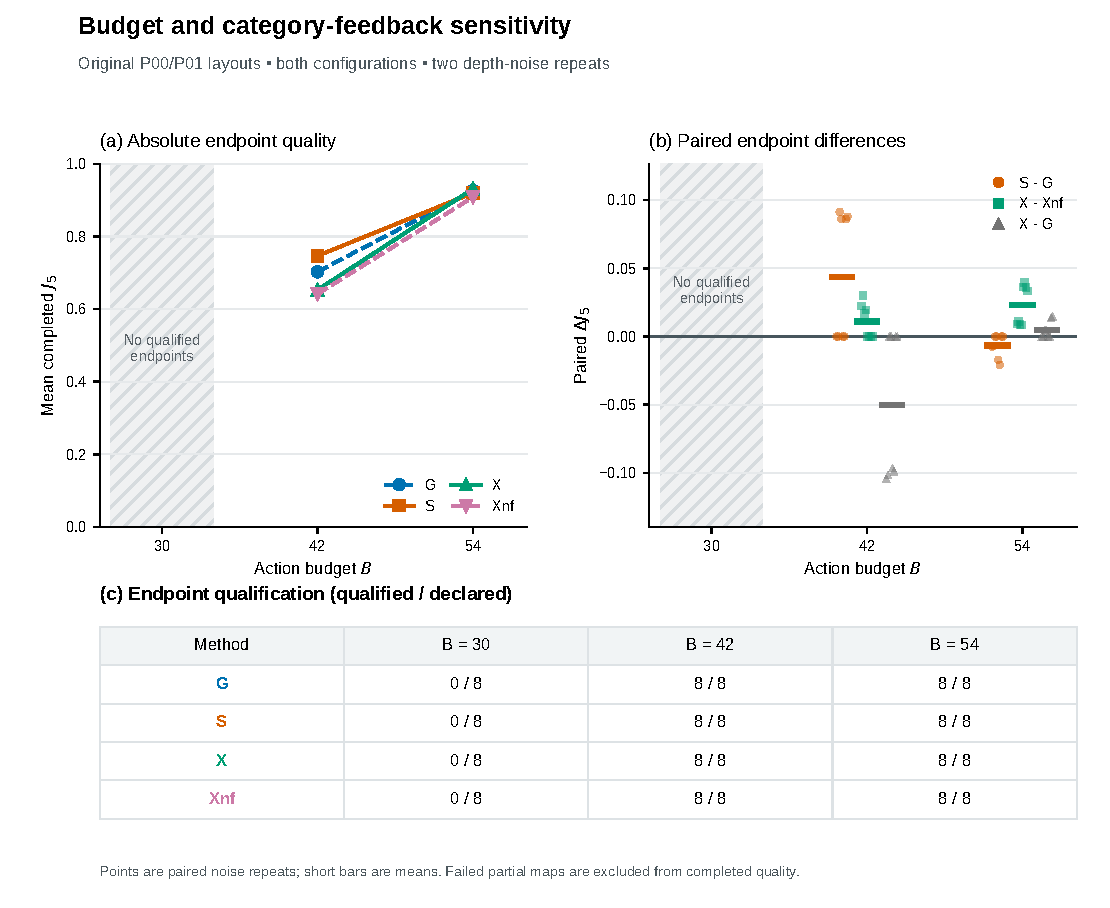
\includegraphics[width=\linewidth,height=.67\textheight,keepaspectratio]{Fig7.pdf}
\caption{Original-layout budget sensitivity. All matched contrasts and qualification counts are retained; budget 30 has no qualified endpoint mean. Short bars indicate complete-pair means rather than confidence intervals across independent scenes}\label{fig:7}
\end{figure}

\hypertarget{separate-multi-facility-extension}{%
\subsection{Separate multi-facility extension}\label{separate-multi-facility-extension}}

A separate implementation places four facilities from two repeated categories in AISLE, CELL, and LOOP layouts, with four nominal structures per instance. It replaces binary dynamic programming with paid observation macros: 0.25 m translation, 30\ensuremath{^{\circ}} rotation, and explicit observation each cost one action. The supplied navigation graph, exact poses, synthetic labels, and structure family remain controlled assumptions. Instances and label planes are inferred from acquired support; full measured depth alone enters TSDF.

Policy names have different meanings here. G uses a uniform structural prior; B mixes uniform and category priors with weight one half; S adjusts that mixture using qualified same-category peers, with leave-one-out evidence; NBV uses geometric myopic scoring without diagnostic lookahead. Thus, local S/G tests category availability, whereas scene-level S/B tests additional sharing. The metric is also separate: \(J_{\rm nav}=C_{\rm nav}(\tfrac14\sum_iF_{1,i})\), using measured-free navigable coverage and all four facilities, including undiscovered ones. Complete predicted meshes are evaluated against fixed observable references without local prediction cropping.

Three controller versions compare the original implementation, measured-floor exclusion from association candidates, and additional same-center nominal-exposure discounting. The latter two are common components for every method; depth fusion is unchanged. Each version declares the same three layouts, four policies, one noise realization, and budget 160. Their values are not pooled with local \(J_5\).

All 36 declared episodes have been attempted, representing three development layouts rather than 36 independent scenes. Every route finishes collision-free with full-pose return. Thirty-five complete their original evaluation pipeline; the remaining original CELL/G failure has a separately derived common-metric result.

\begin{table}[!htbp]
\caption{All 36 scene-level joint scores under a common numerical evaluator. Pipeline success preserves each version's original status}\label{tab:5}
\small\setlength{\tabcolsep}{3pt}
\setlength{\JournalTableWidth}{\dimexpr\linewidth-10\tabcolsep\relax}
\begin{tabular}{@{}>{\raggedright\arraybackslash}p{0.26\JournalTableWidth} >{\raggedright\arraybackslash}p{0.148\JournalTableWidth} >{\raggedright\arraybackslash}p{0.148\JournalTableWidth} >{\raggedright\arraybackslash}p{0.148\JournalTableWidth} >{\raggedright\arraybackslash}p{0.148\JournalTableWidth} >{\raggedright\arraybackslash}p{0.148\JournalTableWidth}@{}}
\toprule
Version/layout & NBV & G & B & S & Pipeline success \\
\midrule
Original/AISLE & 0.856753 & 0.856753 & 0.856753 & 0.856753 & 4/4 \\
Original/CELL & 0.689542 & 0.765328\textsuperscript{a} & 0.766521 & 0.766521 & 3/4 \\
Original/LOOP & 0.620599 & 0.620599 & 0.620599 & 0.620599 & 4/4 \\
Ground/AISLE & 0.652828 & 0.652828 & 0.652828 & 0.652828 & 4/4 \\
Ground/CELL & 0.465491 & 0.533627 & 0.531167 & 0.531167 & 4/4 \\
Ground/LOOP & 0.730488 & 0.730488 & 0.730488 & 0.730488 & 4/4 \\
Exposure/AISLE & 0.782938 & 0.782938 & 0.734222 & 0.734222 & 4/4 \\
Exposure/CELL & 0.515457 & 0.786500 & 0.786500 & 0.786500 & 4/4 \\
Exposure/LOOP & 0.736447 & 0.736447 & 0.690253 & 0.690253 & 4/4 \\
\bottomrule
\end{tabular}
\begin{tablenotes}[flushleft]\footnotesize
\item[a] Original CELL/G completes motion and return but its evaluator rejects a finite triangle of area \(4.24\times10^{-13}\,\mathrm m^2\). The displayed score is a separately derived measurement under the common \(5\times10^{-13}\,\mathrm m^2\) face threshold. It does not replace the original failure status.
\end{tablenotes}
\end{table}

Ground association increases LOOP quality but reduces AISLE and CELL quality. Exposure discounting improves every G endpoint relative to Ground, while B/S decrease in LOOP. Across all three versions, all nine S/B pairs have identical executed actions and endpoint quality. S adjusts confidence in a fixed category distribution rather than learning a new distribution, and two instances per category provide at most one peer. Nonidentical beliefs therefore do not necessarily create actionable sharing. The planned held-out scene-level matrix was not launched because the required S/B behavioral distinction had not been established.

The final version nevertheless exposes two distinct planning mechanisms, detailed in the companion evidence manuscript. AISLE category conditioning changes B's selected target relative to G, followed by an adverse endpoint difference. CELL's diagnostic option changes G's behavior relative to geometric NBV and accompanies a positive endpoint difference. At that diagnostic observation, however, no fresh geometric feedback or posterior update occurs. These are route-policy comparisons; neither difference isolates the effect of a single view or establishes shared-semantic benefit. Complete version-specific routes and component scores remain in the companion evidence manuscript.

\hypertarget{frozen-policy-validation-in-new-background-layouts}{%
\subsection{Frozen-policy validation in new background layouts}\label{frozen-policy-validation-in-new-background-layouts}}

A final protocol fixes two additional layouts before observing results: a side column removes one right-aisle navigation center, while a rear partition interrupts direct rear passage. Both retain the P00 facility family and public templates. The controller, category mapping, sensor noise rule, fusion, evaluation region, 18-action common prefix, and 42-action budget remain unchanged. All legal safe-grid centers are retained; each new layout has 23 centers and 92 oriented poses. The noise seed is the original confirmation seed, so this test adds two background-layout units, not new noise replicates or unseen facility categories. Each layout uses both configurations and G/S, giving eight tasks and four pairs.

All eight tasks complete 42 paid actions and 43 acquired frames, avoid collision, and return to the full initial pose. Table 6 reports every paired endpoint. Mean coverage is identical at 0.934732; mean precision increases from 0.864441 to 0.870224, recall from 0.672455 to 0.704742, and surface F1 from 0.754450 to 0.777445. Mean joint quality increases from 0.705188 to 0.726215, or \textbf{2.9818\%}, with one win and three ties. Relative differences at 2 and 10 cm are 2.8176\% and 3.1200\%. These are descriptive paired results from two new layouts; configurations do not increase the number of independent layout units.

\begin{table}[!htbp]
\caption{All frozen-policy layout pairs at 5 cm. Coverage is equal within each pair; qualification is 8/8}\label{tab:6}
\small\setlength{\tabcolsep}{3pt}
\setlength{\JournalTableWidth}{\dimexpr\linewidth-10\tabcolsep\relax}
\begin{tabular}{@{}>{\raggedright\arraybackslash}p{0.26\JournalTableWidth} >{\raggedright\arraybackslash}p{0.148\JournalTableWidth} >{\raggedright\arraybackslash}p{0.148\JournalTableWidth} >{\raggedright\arraybackslash}p{0.148\JournalTableWidth} >{\raggedright\arraybackslash}p{0.148\JournalTableWidth} >{\raggedright\arraybackslash}p{0.148\JournalTableWidth}@{}}
\toprule
Layout / config. & Coverage & G F1 & S F1 & G joint & S joint \\
\midrule
Side column / h0 & 0.954145 & 0.806490 & 0.806490 & 0.769508 & 0.769508 \\
Side column / h1 & 0.955908 & 0.702575 & 0.702575 & 0.671597 & 0.671597 \\
Rear partition / h0 & 0.914439 & 0.806490 & 0.806490 & 0.737485 & 0.737485 \\
Rear partition / h1 & 0.914439 & 0.702246 & 0.794224 & 0.642160 & 0.726269 \\
Mean & 0.934732 & 0.754450 & 0.777445 & 0.705188 & 0.726215 \\
\bottomrule
\end{tabular}
\end{table}

Figure 8 shows all saved paths. In the side-column layout, both initial observation directions satisfy the return constraint. Category information changes candidate values but does not change their ordering: both methods choose left and remain identical in actual actions. In the rear-partition h1 condition, G's initial left/right values tie within the frozen numerical tolerance; its original ordering selects left, whereas S selects right. Their nonsemantic histories and geometric log odds are identical at step 18; category weights alone differ. The first executed divergence is action 19, followed by greater recovered surface recall at unchanged coverage. This supports the complete category-conditioned route's effect, not a separate quality gain attributable to a single frame.

\begin{figure}[!htbp]
\centering
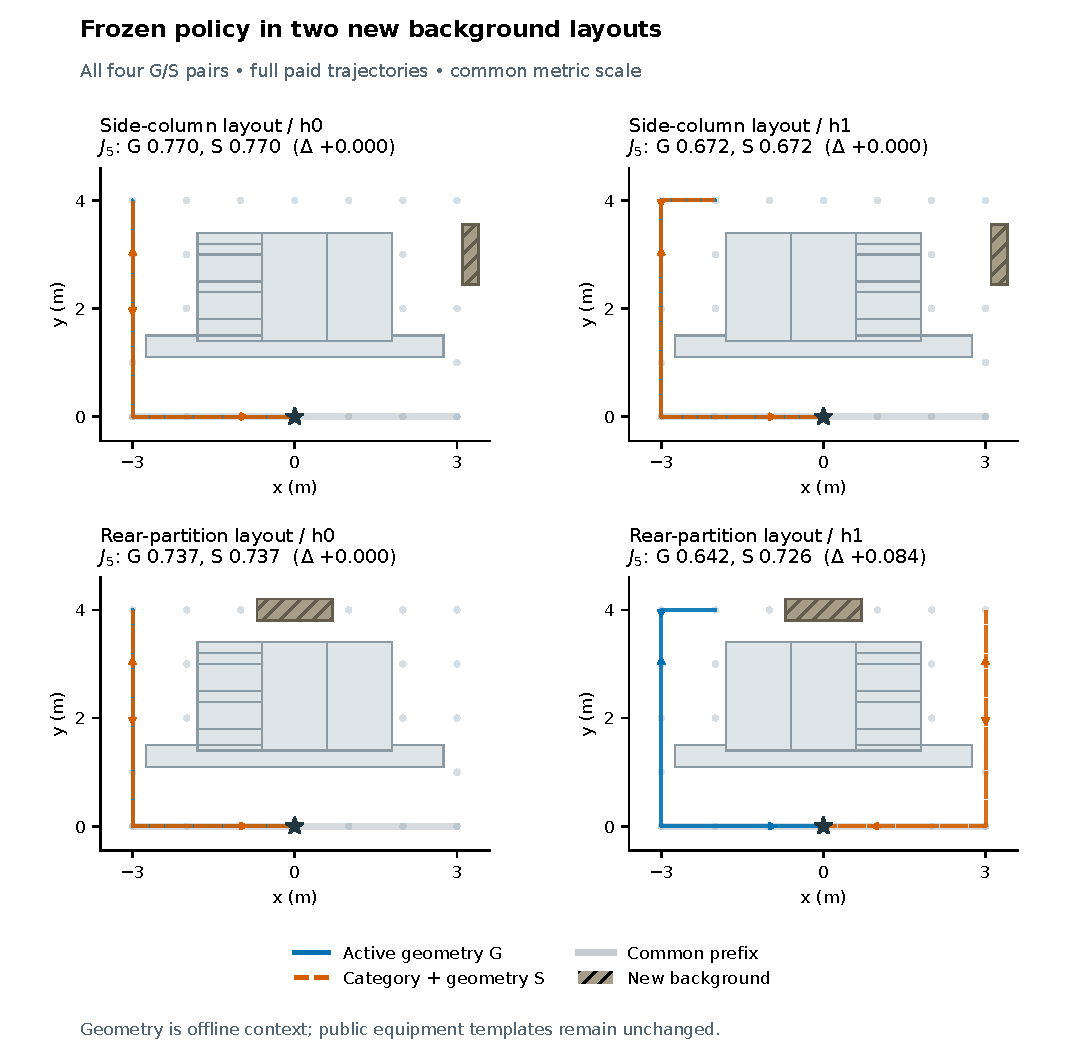
\includegraphics[width=\linewidth,height=.67\textheight,keepaspectratio]{Fig8.pdf}
\caption{Complete paths of all four new background-layout pairs, with recorded headings and a common metric scale. Gray marks the shared paid prefix; hatched regions show added background structures outside the unchanged facility evaluation region. Geometry supplies offline context. Three pairs coincide, while rear-partition h1 diverges at action 19. The companion evidence includes all eight actual endpoint meshes and quality components}\label{fig:8}
\end{figure}

G/S mean travel is 27.0/26.5 m, with 15.0/15.5 turns. Single-thread planning wall time averages 0.0474/0.0484 s per task on an Intel Xeon processor (Sapphire Rapids); complete task times, including sensing, fusion and evaluation, range from 5.0 to 5.8 s. Timing is descriptive for this four-logical-CPU host, not a real-time or cross-hardware benchmark. Independent review checks all 344 saved frames, priors, measured residuals, selected actions, return constraints, source hashes and endpoint arithmetic. No parameters are retuned after these results, and no reserved additional tasks are used.

\hypertarget{discussion-and-conclusion}{%
\section{Discussion and Conclusion}\label{discussion-and-conclusion}}

The demonstrated local mechanism is an early directional choice under budget pressure. Category support changes the first autonomous action and improves side-surface recovery without more actions, frames, or travel. Checkpoints connect that choice to measured recall and F1; the extension tests its persistence under new noise and same-family changes. Neither establishes broad unseen-scene generalization.

Both h0 conditions tie; the lowest budget fails the feasibility test; the highest budget reverses policy ordering. The analysis assumes correct utilities, whereas the controller uses an exposure surrogate, so it does not predict that reversal. Public templates, synthetic cues, exact poses, and a supplied safe graph simplify perception and navigation. Natural recognition, estimated-pose SLAM, temporal map maintenance, and dynamic avoidance remain untested. The available ROS 1 platform supports future deployment work but adds no physical performance evidence.

Cross-instance sharing remains a separate, unproven benefit. An earlier, distinct six-parent shared-reliability development study also gives five nominal S/G ties and one loss, with a \ensuremath{-}0.3301\% relative mean difference; mismatched-relation S/B comparisons all tie. That incomplete matrix and its different controller/metric are retained in supplementary evidence, not pooled with the present results. Increasing semantic model complexity is therefore not itself an empirical contribution.

Overall, the study supports a conditional application result: category information improves mean local joint quality by 6.1638\% in the original confirmation, and the complete correction policy provides a 2.6241\% development improvement. The frozen-policy test adds a 2.9818\% mean gain across two new background layouts, with one win and three ties. Budget and geometry tests establish where these results persist and where they do not. Further progress should align predicted observation value with measured surface quality before claiming general multi-facility gains or transferring the full method to physical operation.

\hypertarget{reproducibility-and-data}{%
\section{Reproducibility and Data}\label{reproducibility-and-data}}

The complete evidence manuscript (Online Resource 4) and supplementary methods (Online Resource 5) retain implementation equations, settings, version boundaries, and evidence links. Archived sources, input manifests, observations, actions, meshes, and plotting provenance support reproduction. All 128 extension records, 36 scene-level attempts, and eight final layout-validation tasks remain available with failures distinguished; reconstruction checkpoints reuse saved observations. The final validation retains a preregistered configuration, archived implementation, sealed packets and meshes, and independent frame-level review. A representative 43-frame saved replay reproduces its controller, maps and meshes exactly without new sensing; an offline interactive demonstration accompanies the reproducibility index.

\begin{thebibliography}{99}
\bibitem{ref9} World Economic Forum. Physical AI: Powering the New Age of Industrial Operations. White paper, 2025-09-04. \href{https://www.weforum.org/publications/physical-ai-powering-the-new-age-of-industrial-operations/}{Official white paper}.

\bibitem{ref10} Placed J. A., Strader J., Carrillo H., Atanasov N., Indelman V., Carlone L., Castellanos J. A. A Survey on Active Simultaneous Localization and Mapping: State of the Art and New Frontiers. IEEE Transactions on Robotics, 2023. \url{https://doi.org/10.1109/TRO.2023.3248510}.

\bibitem{ref1} Chaplot D. S., Gandhi D., Gupta S., Gupta A., Salakhutdinov R. Learning to Explore using Active Neural SLAM. ICLR, 2020. Author manuscript: \url{https://doi.org/10.48550/arXiv.2004.05155}.

\bibitem{ref5} Cao C., Zhu H., Choset H., Zhang J. TARE: A Hierarchical Framework for Efficiently Exploring Complex 3D Environments. RSS, 2021. \url{https://doi.org/10.15607/RSS.2021.XVII.018}.

\bibitem{ref6} Chen X., Li Q., Wang T., Xue T., Pang J. GenNBV: Generalizable Next-Best-View Policy for Active 3D Reconstruction. CVPR, 2024:16436--16445. \url{https://doi.org/10.1109/CVPR52733.2024.01555}.

\bibitem{ref4} Zhou Q.-Y., Park J., Koltun V. Open3D: A Modern Library for 3D Data Processing. arXiv:1801.09847, 2018. \url{https://doi.org/10.48550/arXiv.1801.09847}.

\bibitem{ref11} Curless B., Levoy M. A Volumetric Method for Building Complex Models from Range Images. Proceedings of SIGGRAPH, 1996:303--312. \url{https://doi.org/10.1145/237170.237269}.

\bibitem{ref2} Dharmadhikari M., Alexis K. Semantics-aware Exploration and Inspection Path Planning. ICRA, 2023. \url{https://doi.org/10.1109/ICRA48891.2023.10160469}.

\bibitem{ref7} Dharmadhikari M., Alexis K. Semantics-Aware Predictive Inspection Path Planning. IEEE Transactions on Field Robotics, 2025. \url{https://doi.org/10.1109/TFR.2025.3578402}.

\bibitem{ref3} Nagami K., Chen T., Yu J., Shorinwa O., Adang M., Dougherty C., Cristofalo E., Schwager M. VISTA: Open-Vocabulary, Task-Relevant Robot Exploration With Online Semantic Gaussian Splatting. IEEE Robotics and Automation Letters, 11(3):3150--3157, 2026. \url{https://doi.org/10.1109/LRA.2026.3653276}.

\bibitem{ref8} Chen L., Zhan H., Yin H., Xu Y., Mordohai P. Understanding while Exploring: Semantics-driven Active Mapping. Advances in Neural Information Processing Systems, 38, 2025. \url{https://doi.org/10.52202/085713-1113}.

\bibitem{ref12} Kaelbling L. P., Littman M. L., Cassandra A. R. Planning and Acting in Partially Observable Stochastic Domains. Artificial Intelligence, 101(1--2):99--134, 1998. \url{https://doi.org/10.1016/S0004-3702(98)00023-X}.

\bibitem{ref13} Hollinger G. A., Sukhatme G. S. Sampling-based Robotic Information Gathering Algorithms. The International Journal of Robotics Research, 33(9):1271--1287, 2014. \url{https://doi.org/10.1177/0278364914533443}.

\bibitem{ref14} Knapitsch A., Park J., Zhou Q.-Y., Koltun V. Tanks and Temples: Benchmarking Large-Scale Scene Reconstruction. ACM Transactions on Graphics, 36(4), 2017. \url{https://doi.org/10.1145/3072959.3073599}.
\end{thebibliography}

\section*{Statements and Declarations}
\subsection*{Funding}
\textit{Author confirmation required:} \underline{\hspace{5cm}}
\subsection*{Competing interests}
\textit{Author confirmation required:} \underline{\hspace{5cm}}
\subsection*{Author contributions}
\textit{Author confirmation required:} \underline{\hspace{5cm}}
\subsection*{Data and code availability}
See the Reproducibility and Data section and the accompanying Online Resources.
The final public version identifier and any access restrictions require author confirmation.
\subsection*{AI assistance disclosure: draft for author confirmation}
OpenAI Codex assisted with manuscript organization and revision and with developing
experiment, analysis, and plotting code. Tool/model versions, the extent of assistance,
and the authors' verification and responsibility statement must be completed before submission.
This draft disclosure does not assert that the authors have already approved the manuscript.

\subsection*{Online Resources}
Online Resource 1: matched detail views (\texttt{ESM\_1.pdf}).

Online Resource 2: Complete precision/recall figure (\texttt{ESM\_2.pdf}).

Online Resource 3: actual stage meshes (\texttt{ESM\_3.pdf}).

Online Resource 4: complete evidence manuscript (\texttt{ESM\_4.pdf}).

Online Resource 5: supplementary methods (\texttt{ESM\_5.pdf}).
\end{document}
